\documentclass{article}
\usepackage[spanish]{babel}
\usepackage{graphicx}
\usepackage[utf8]{inputenc}
\usepackage[spanish]{babel}
\usepackage{natbib}
\usepackage{float}
\usepackage{amsmath}
\usepackage{amssymb}
\usepackage{array}
\usepackage{booktabs}
\usepackage{tikz}
\usetikzlibrary{shapes.geometric, arrows}

\tikzstyle{startstop} = [rectangle, rounded corners, minimum width=3cm, minimum height=1cm,text centered, draw=black, fill=red!30]
\tikzstyle{process} = [rectangle, minimum width=3cm, minimum height=1cm, text centered, draw=black, fill=orange!30]
\tikzstyle{decision} = [diamond, minimum width=1.5cm, minimum height=0.8cm, text centered, draw=black, fill=green!30,font=\footnotesize]
\tikzstyle{arrow} = [thick,->,>=stealth]
\title{Clasificación inteligente sinergia entre lógica difusa y algoritmos genéticos }
\author{José Adrián Rodríguez González}
\date{Noviembre 2024}
\begin{document}
\maketitle
\section{Introducción}
Para este mes, se corrigió el primer modelo que se tenía, sin embargo, para poder corregir los errores, se desarrolló otro modelo con una mira distinta.
\section{Problema del Iris.}
Este conjunto de datos es uno de los más clásicos, consiste en 3 especies de flores, cada una posee 4 características.
\begin{figure}[h]
    \centering
    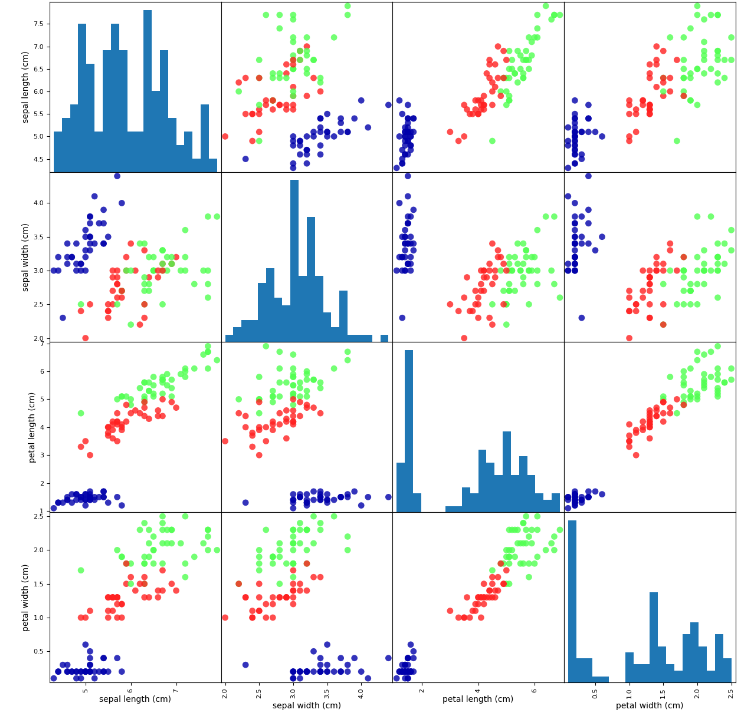
\includegraphics[width=0.5\textwidth]{image.png}
    \caption{Cruza y mutación}
    \label{fig:fig1}
\end{figure}

Este problema se basa del paper de \citep{413232}, en el que usa este conjunto de datos para probar su selección. En este caso, se siguió el proceso descrito del mes pasado, solamente que se cambió la forma de clasificar, anteriormente lo que se realizaba era separar las clases dentro del conjunto de prueba de salida para calcular los \(\alpha\), sin embargo, las clases como se mencionó en octubre dependen de la clase asociada a la regla máxima,así que se cambió el proceso.Con este enfoque Michigan se puede clasificar la clase sin tener que ponderarse a una punto. Los procesos del algoritmo genético cambiaron, ahora se realiza una selección por torneo, la cruza es a través de una máscara binaria,en la que se intercambia aleatoriamente el indice de los dos padres.
La mutación, utiliza un 0.1 de tasa y compara los hijos con los padres para observar quienes son los individuos que se quedan para la siguiente generación. Además, se añadió el subconjunto \textit{Don't care}, que es una forma de reducir la cantidad de patrones en nuestro sistema basado en reglas.
Sin embargo, el problema que se observó en este modelo, es que convergía a las pocas generaciones.
Para evitar que convergiera tan rápido el modelo se reintroduce una población aleatoria cada cierta generación
Se probo con 1000 individuo por 20 generaciones, y a las pocas generaciones tendían a una regla. Sin importar las formas en como se ejecutaba el experimento, siempre convergía al conjunto [0,0,2,0] con un CF de 1, para la clase 1, y las reglas [0,0,5,0], con un CF de 0.8678 y clase de 3, y [0,0,4,4], para la clase 2.

\begin{table}[h!]
    \centering
    \begin{tabular}{@{}cccc@{}}
    \toprule
    \textbf{Regla}       & \textbf{Fitness} & \textbf{CF (Factor de Confianza)} & \textbf{Clase} \\ \midrule
    {[0, 0, 5, 0]}       & 8                & 0.8678                            & 3              \\
    {[0, 0, 2, 0]}       & 8                & 1.0000                            & 1              \\
    {[0, 0, 4, 4]}       & 3                & 0.7149                            & 2              \\ \bottomrule
    \end{tabular}
    \caption{Resumen de las mejores reglas.}
    \label{tab:best_rules}
\end{table}
%70 accuracy
Los individuos se repiten muchas veces, por lo que se necesitará realizar otro tipo de estrategias. 
Una de las métricas que se utilizó para medir la eficiencia del modelo fue el accuracy y, particularmente como lo menciona \Citep{413232}, el modelo puede sobre ajustarse, dando un accuracy o muy cercano al 100\%. En nuestro modelo propuesto, dió un accuracy de 99\%, lo que puede significar que nuestro modelo se sobreajusta a nuestro conjunto de datos, por lo que sería punto de estudio, el usar validaciones cruzadas o \textit{Leaving one out}, como técnica para corrobar y poder corregir el sobreajuste de nuestro modelo 
\section{Conclusión}
Después de haber mejorado el modelo con las otras estrategias, se implementará en el modelo para la base de datos de cáncer de mama.
\bibliographystyle{apalike}
\bibliography{reference}
\end{document}